
\section{Methods}
\label{sec:DOICollectionMethods}
Initially, we assume that our eye-tracking experiments will use visualizations which are accessible for instrumentation to programmers. Thus, graphical information (e.g. position, size, shape) of internal visualization primitives (e.g. circles representing nodes in a graph) are available at rendering time. 

Our proposed methods will only operate over visualizations with open source-code. This is a limitation of our work. However, we claim that open source code libraries are gaining popularity over proprietary applications. Figure~\ref{fig:WebUsageChart} shows a comparison between two popular visualization libraries: d3JS (open source-code) and FusionChart (proprietary application).

\begin{figure}[htb]
  \centering
  \includegraphics[width=0.99\linewidth]{images/WebUsageChart.eps}
  \caption{: Comparison of number websites using d3js and FusionChart in their homepages. Data collected from http://trends.builtwith.com/. }
	\label{fig:WebUsageChart}
\end{figure}

We aim to map gazes to visualization primitives using our viewed-object-detection algorithm. Our algorithm will seek to compute ``object viewing scores'' that express the likelihood that an object is viewed given a particular gaze sample. The viewed-object-detection algorithm outputs object viewing scores from which we can construct DOI data. We aim to develop viewed-object-detection algorithm incrementally in three stages. First, we plan to detect objects using the na�ve approach of AOI binning. We will consider each visual object as an AOI. In this method, the objects where most recent gazes landed will be considered as `viewed'. Second, we intent to develop a method for calculating a probabilistic fuzzy score for each object based on the proximity of gaze landing to the object. Third, we plan to build on Salvucci's method~\cite{Sal00} to develop an algorithm to calculate the object viewing score based on the probabilistic score and an additional prediction score. The prediction score will be calculated based on the semantic content in the data. 

\begin{figure}[htb]
  \centering
  \includegraphics[width=0.99\linewidth]{images/System.eps}
  \caption{: Detection of viewed objects in generative visualizations.}
	\label{fig:System}
\end{figure}

We depict our general approach for collecting DOI data in Figure~\ref{fig:System}. Eye-trackers supply gaze samples in screen space. The `Screen to Model Transformation' module (Figure~\ref{fig:System}) will transform these gaze samples to the visualization model space. The `Renderer' module will render the visualization, and supply information regarding shapes and positions of visual objects, and model transform information. Afterward, our algorithm will combine gaze samples and visual object positions to detect viewed objects by calculating object-viewing-scores. A prediction module will use information about what a user has viewed in the past and interacted with, to infer what objects the user is likely to be viewing presently. In Figure~\ref{fig:System}, we can see that gaze position and visualization information is passed to the viewed object detection module. We hypothesize that this will reduce the inaccuracies previously illustrated, by allowing us to discriminate which visual object is users is likely to be looking at, when gazes land near multiple objects.
More details about the three stages of developing viewed-object-detection algorithm are provided below. 

\subsection{AOI-based viewed object detection}
\label{sec:AOIBasedViewedObjectDetection}

A na\"{\i}ve approach is to treat object shapes as dynamic AOIs and determine that a viewed object is that with the most recent fixation landing in its AOI. Manually drawn AOIs are typically used in the same manner in offline eye-tracking data analysis, and the similar concept of objects of interest (OOIs) has been proposed already by Stellmach et al.~\cite{Ste10} for generative 3D content.

The problem with this approach is that for highly granular visual content, such as individual nodes or labels, users often fixate in the vicinity of the object rather than on the object itself. A potential solution is to pad object AOIs to be slightly larger than the objects. However, larger AOIs may lead to overlap in cluttered visualizations. We demonstrate and quantify these observations in Section~\ref{sec:DOICollectionEvaluation}. Ultimately, the problem lies with an inability to determine with absolute certainty what a user is looking at, and is described in more detail in the next section.

\subsection{A probabilistic approach to viewed object detection}
\label{sec:ProbabilisticObjectDetection}

Unlike mouse input, eye-tracking can only indicate a small screen region that a user is fixating, rather than a particular pixel. Typically, such regions are about one inch in diameter, though specific values depend on viewing conditions. As such, it is generally impossible to tell with certainty which object a user is viewing, if the user is fixating in the vicinity of multiple close objects (Figure~\ref{fig:discreminateFig4}(a)). This is not a significant problem for traditional AOI analyses, which generally use large AOIs. Conversely, we aim to detect the viewing of granular visual content, such as network nodes or glyphs, in cluttered visualizations.

\begin{figure}[htb]
  \centering
  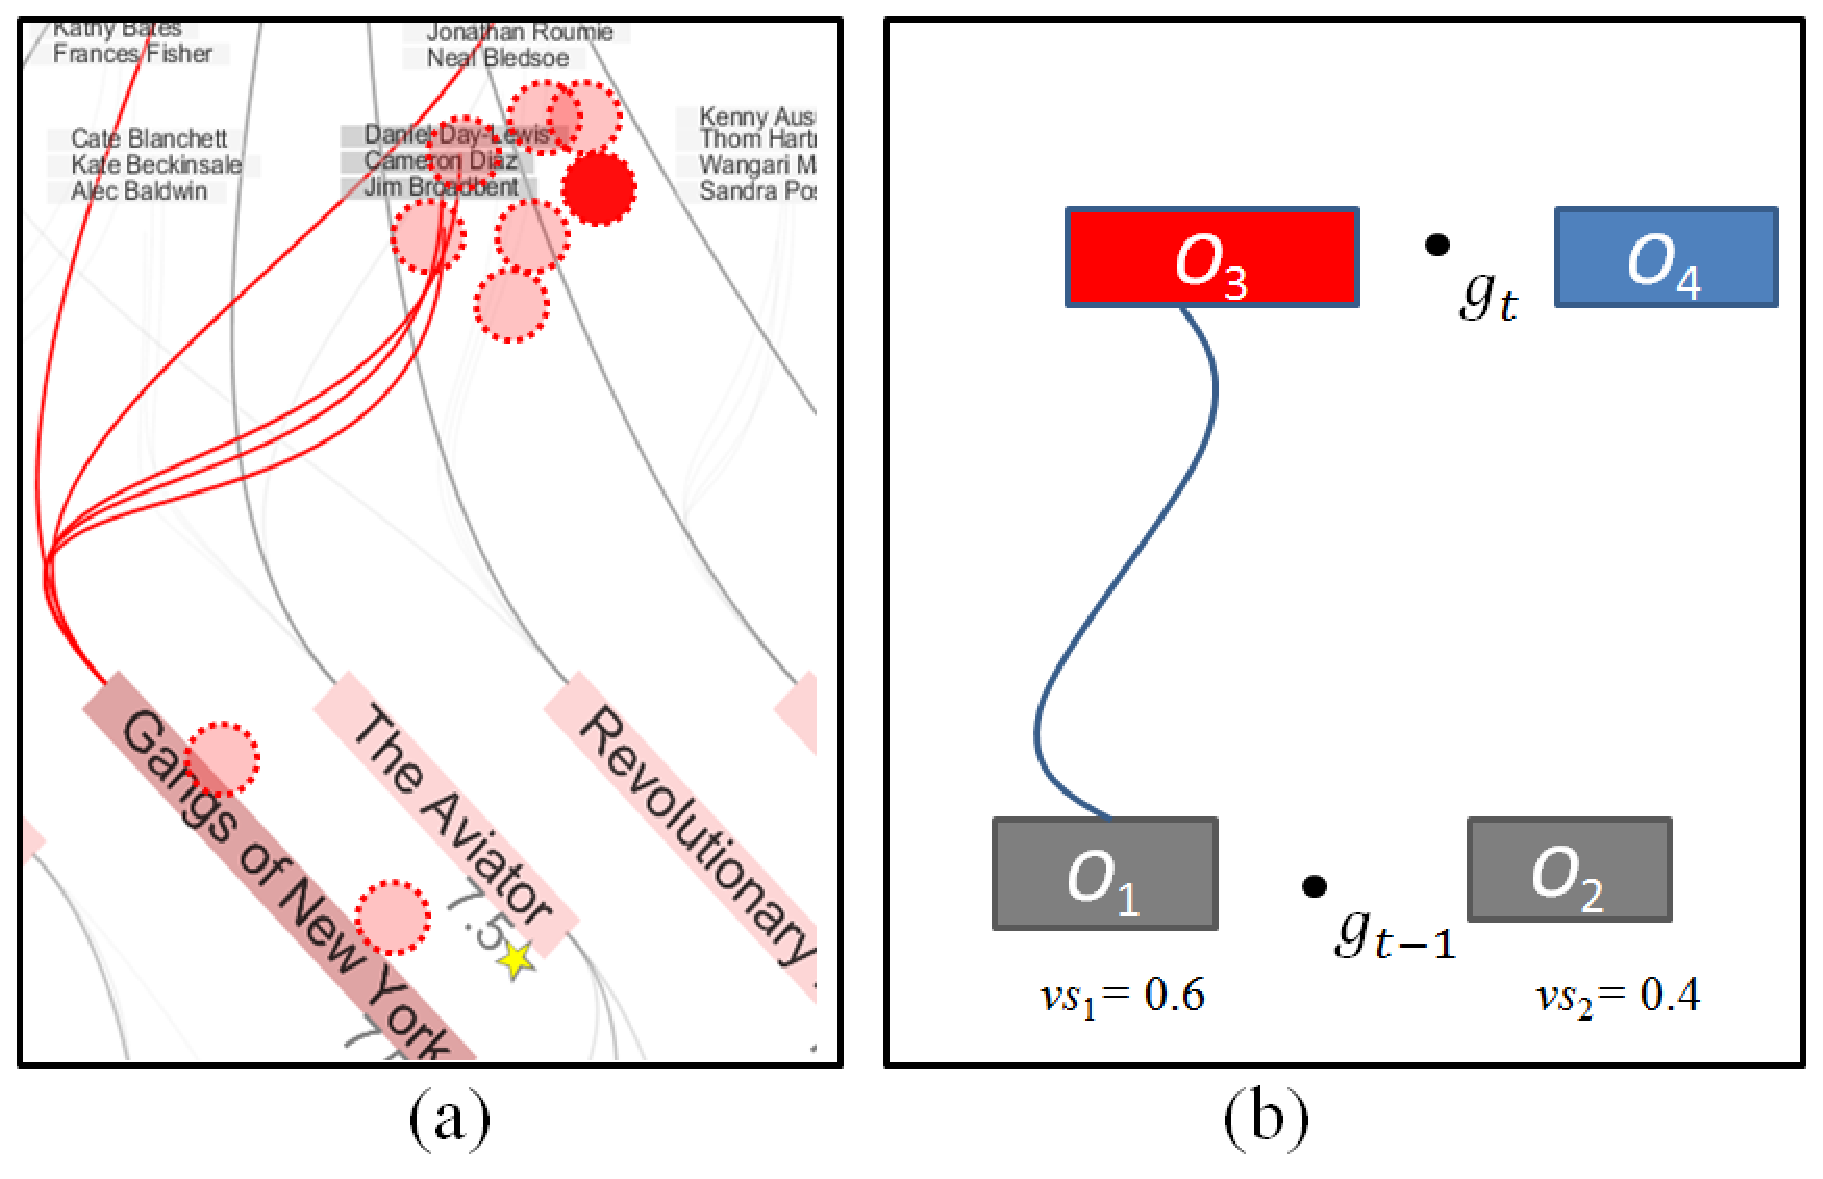
\includegraphics[width=\linewidth]{images/discreminateFig4.eps}
  \caption{(a) A real visualization example in which a user fixates in the vicinity of multiple close object groups (red dot). (b) predictive method: even though the latest gaze sample falls equidistantly between visual objects $O_3$ and $O_4$, we suspect that $O_3$ is the more likely viewing target given that it is highlighted and connected to $O_1$, which is likely to have been the object that the user viewed previously ($vs_1=0.6 > vs_2 = 0.4$). }
	\label{fig:discreminateFig4}
\end{figure}

We advocate for a fuzzy interpretation of gaze data and detect likelihoods that objects are viewed rather than certainties. To this end, we can compute object gaze scores $gs$ (for all objects $i$ in a visualization, and at all times $t$) that range between zero- the object is not viewed, and one- the object is certainly viewed, as shown in Figure~\ref{fig:gazeScoreFig3} and Formula~\ref{eq:GS}. 

\begin{figure}[htb]
  \centering
  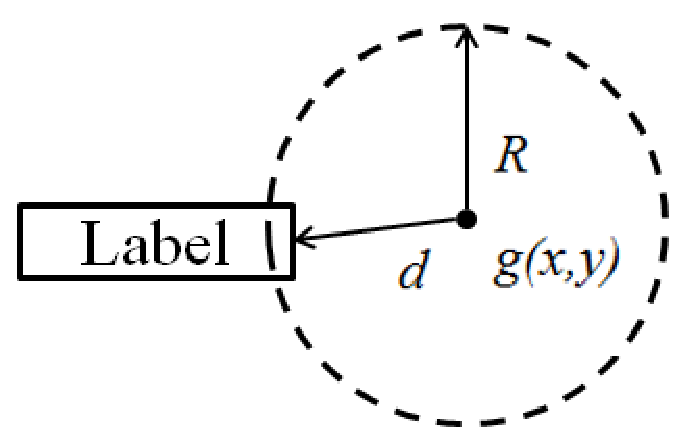
\includegraphics[width=0.4\linewidth]{images/gazeScoreFig3.eps}
  \caption{Calculating gaze score $gs$ for a gaze sample landing near an object. $d$ is the distance from the object to the gaze sample, and $R$ approximates the size of the user's foveated region.}
	\label{fig:gazeScoreFig3}
\end{figure}

%Formula 1
\begin{equation}
gs_{i,t} = 1 - \min (1, (\frac{d}{R}))
\label{eq:GS}
\end{equation}

The region of radius $R$ used in the formula is analogue to the user's foveated region, and as such needs to be constant in screen space. Thus, if the view is zoomed in or out, $R$ needs to be scaled accordingly in model space to remain constant in screen space.  Similar approaches were used by Salvucci et al.~\cite{Sal00} and Okoe et al.~\cite{Okoe14}.

Finally, we note that the object scores ($gs$) do not directly equate to probabilities. The distinction is important because our implementation can detect two objects as being viewed simultaneously ($gs_1 = 1$ and $gs_2=1$). We think this is appropriate since a person can in fact visually parse multiple objects at the same time if they fall within the user's foveated region, and even think of multiple objects as a unit for specific task purposes.



\subsection{A predictive algorithm for viewed object detection}
\label{sec:MehthodsIntelligentAlgorithm}

Salvucci and Anderson described the concept of ``intelligent gaze interpretation'' in the context of a gaze-activated interface ~\cite{Sal00}. They more accurately detected which interface control a user was gazing at, by integrating both the proximity of the gaze to the control, and the likelihood that the control was the target of a gaze-interaction, based on the current state and context of the interface. Formally, their algorithm identified the most likely currently viewed item $i_{viewed}$ by solving

\begin{equation*}
i_{viewed} = \displaystyle \argmax_{i\in I}%[Pr(g|i)\cdot Pr(i)]
\end{equation*}

where $Pr(g|i)$ is the probability of producing a gaze at location $g$ given the intention of viewing item $i$, and $Pr(i)$ is the prior probability of an item $i$  being the target of a gaze-interaction. Salvucci and Anderson based these prior probabilities on assumptions about how an interface might be used, and hardcoded them into their system.  

We adapt Salvucci and Anderson's paradigm to solve the ambiguous case when a gaze-sample lands close to multiple objects (e.g.,  Figure~\ref{fig:discreminateFig4}(a)). For example, in a network visualization we may assume that a user who has just viewed a node $n$ will more likely view one of $n$'s neighbors than a random other node, perhaps especially if the user previously highlighted node $n$ and its outgoing edges.  In Section~\ref{sec:DOICollectionEvaluation} we show quantitatively that this assumption holds for one tested visualization.  

We consider the simplified scenario in Figure~\ref{fig:discreminateFig4}(b): four visual objects ($O_{1\ldots 4}$), two of which are connected ($O_1$ and $O_3$), and one of which is highlighted ($O_3$), are shown on the screen. A new gaze sample registers between $O_3$ and $O_4$ at time $t$. Intuitively, it is more likely that $O_3$ was viewed since it is highlighted. Moreover, if we knew that $O_1$ was viewed just before the current moment  and assume that users generally view neighboring nodes together, then this likelihood becomes stronger.         
 
Formally, we compute $vs_{i,t}$  (i.e., the viewing score $vs$ of object $i$ at time $t$) by weighing the gaze score $gs_{i,t}$ described in Section~\ref{sec:ProbabilisticObjectDetection} by a prediction score $ps_{i,t}$ that object $i$ is a viewing target at time $t$:  
%Formula 2
\begin{equation}
vs_{i,t} = gs_{i,t} \times ps_{i,t}
\label{eq:VS}
\end{equation}

This prediction score is computed based on the likelihood that an object is viewed if another object (e.g.,  a node's neighbor) was viewed just before it. Specifically, $ps$ is derived from a viewing transition function $T$ between objects:  $T(j,i)$ gives the likelihood that object $i$ is viewed after object $j$ is viewed. We will assume that $T(j,i)$ is given as input to our algorithm. Concrete examples of what $T(j,i)$ could be linked to are whether objects $i$ and $j$ are somehow connected or related, or whether they are part of a special group (e.g., highlighted elements). Moreover, connections could be either visual, such as an explicit edge or leader line or an implicit sharing of similar visual attributes (e.g., color, shape), or semantic (e.g., both nodes are actors). More examples of $T(j,i)$ functions, and means of defining them, are described throughout the paper.

To compute $ps$, we could consider $ps_{i,t} = T(j,i)$ but that would involve knowing $j$, the previously viewed object, with absolute certainty. As exemplified in Figure~\ref{fig:discreminateFig4}(b), we often cannot unequivocally determine which item was viewed at a given time: $O_1$'s previous viewing score ($vs_{1,t-1}=0.6$), is just slightly larger than $O_2$'s viewing score ($vs_{2,t-1}=0.4$), and thus an absolute choice of $O_1$ over $O_2$ as previously viewed element would be rather arbitrary.  In other words, we cannot say with absolute certainty which of the two objects was viewed before because the user fixated between them. 

In more general terms, our computation of $ps_{i,t}$ must account for multiple items $j$ that may have been viewed before. These items $j$ are those with a previous visual score $vs_{j,t-1}$ that is greater than $0$.  As such, we compute $ps_{i,t}$ as a weighted average of all transition probabilities from objects $j$ with $vs_{j,t-1} > 0$ , to our current item $i$. The weights are given by the likelihood that an object $j$ was viewed before - in other words by its previous viewing score $vs_{j,t-1}$. This computation is captured by Formula~\ref{eq:ps}.  

%Formula 4
\begin{equation}
ps_{i,t} = \frac{\displaystyle\sum_{j} {vs_{j,t-1} \times T(j,i)}}{\displaystyle\sum_{j} vs_{j,t-1}} \text{ , where  } \parbox{15em}{$0\leq i \leq n$ and $gs_{i,t} > 0$\\$0\leq j \leq n$ and $vs_{j,t-1} > 0 $\\ $0\leq j \leq n$ and $gs_{j,t} = 0$ }
\label{eq:ps}
\end{equation} 

Finally, an important constraint needed to be added to Formula~\ref{eq:ps}. Intuitively, our approach means that previously viewed objects $j$ act as referees with varying degrees of influence (i.e., previous visual scores) in a competition between currently viewed items $i$. This analogy provides the intuition for the necessary constraint: an object should not referee a competition that it is part of. For example, in our simplified scenario, using $O_3$ as a previous element in a competition between itself and $O_4$ would result in an open feedback-loop and should be avoided. This restriction is reflected in Formula~\ref{eq:ps} by the 3rd inequality.  The algorithm pseudocode is provided below.

\begin{algorithm}
\caption{Viewed Object Detection Algorithm}
\label{alg:ObjectDetection}
\begin{algorithmic}[1]
\State \textbf{Inputs: } 
\Statex $O_{i, \ldots, n}$= tracked visualization objects (shapes, positions)
\Statex $g(x,y) = $ gaze sample in model space (time $t$)
\Statex $T(i,j) = $ viewing transition function ($T(i,j) \in [0,1]$)
\State \textbf{Outputs:}
\Statex $vs_{i,t} = $ momentary viewing scores of all objects ($i = 1, \ldots, n$). 
\For{$i \gets 1 \text{ to } n$}
	\State Compute $gs_{i,t}$	using Formula~\ref{eq:GS}
\EndFor
\State $max \gets 0$
\For{$i \gets 1 \text{ to } n$}
	\If{$gs_{i,t} > 0$} \label{algLine:PredictionScoreLines}
		\State Compute $ps'_{i,t}$	using Formula~\ref{eq:ps}
		\If{$ps'_{i,t} > max$}
			\State $max \gets ps'_{i,t}$
		\EndIf
	\EndIf
\EndFor
\For{$i \gets 1 \text{ to } n$}
	\State $vs_{i,t} \gets gs_{i,t} \times \frac{ps'_{i,t}}{max} $
\EndFor
\end{algorithmic}
\end{algorithm}

Last, we note that to optimize for speed, we only compute prediction scores for objects with non-zero gazes (Algorithm~\ref{alg:ObjectDetection}, line~\ref{algLine:PredictionScoreLines}). Also, we compute viewing scores for every gaze sample, rather than every fixation. We believe that doing so leads to results that are less dependent on how fixations are computed and more robust. Since our eye-tracker's sampling rate is $120$Hz, the scores $vs_{j, t-1}$ were computed just $8$ms ago, an interval generally shorter than the time it takes for people to shift their attention to a new object. As such, instead of using the raw $vs_{j,t-1}$ score, we use an average of the last several viewing scores, and, for all practical purposes, the term $vs_{j,t-1}$ should be replaced in the previous formulas by $ \sum_{k=1}^{k=15}{vs_{j,t-1}}$, which, given our eye-tracker's $120$Hz temporal resolution, averages samples over approximately $125$ms, a time window we observed to be close to an average fixation duration.  However, we note that our algorithm can take as input fixations rather than individual gaze samples, in which case this step would not be necessary. Moreover, additional smoothing and filtering such as those summarized by Kumar et al.~\cite{Kum08} could be used to clean gazes before feeding them into our algorithm. We tried removing gaze samples with high velocity as they are likely to be part of saccades, but observed no discernable improvement in our algorithm's output. 


{\bf Performance analysis:} The algorithm swifts through all objects ($n$) to find those in the proximity of a gaze sample or fixation ($k_t$). Then, to compute $ps$ for each of the $k_t$ potentially viewed elements, the algorithm iterates over $k_{t-1}$ objects with non-zero viewing scores from the previous iteration. The algorithm is linear if we consider the number of objects that a user can view at any time to be a constant. This is not true for example if the visualization is zoomed out too much and falls entirely within the algorithm's $R$ radius. However, in such cases the output of the algorithm would be meaningless anyway and the algorithm should be aborded.